\section{สรุป}

อ้างอิงจาก \cite[Interference Coordination Method for Integrated HAPS-Terrestrial Networks]{liu2021interference}

การใช้งาน HAPS และ TN ร่วมกันจะต้องคำนึงถึง interference ระหว่างระบบ
วิธีที่มีการนำเสนอคือ ให้พิจารณาการกระจาย traffic load และความพร้อมในการให้บริการของ
HAPS และ TN ใน coverage area

\begin{itemize}
    \item พื้นที่ที่ไม่มีการ overlap กันระหว่าง HAPS และ TN จะไม่มีการประสานการทำงาน
    \item พื้นที่ที่มีการ overlap กันระหว่าง HAPS และ TN จะมีการให้บริการโดย (ก.) HAPS หรือ TN หรือ (ข.) ทั้ง HAPS และ TN
            โดยพิจารณาจากปัจจัยที่กำหนดจะมีการกำหนดขึ้นเพื่อให้เกิด throughput สูงสุด
\end{itemize}

พื้นที่ที่ไม่มี traffic load จะเปลี่ยนสถานะของ HAPS beam หรือ TN base station ไปเป็น idle เพื่อประหยัดการใช้พลังงาน

\section{ความเห็นของนิสิต}

\begin{multicols}{2}
\begin{minipage}{0.4\textwidth}
\textbf{\authorAName}:\\
การแทรกสอดการทำงานระหว่าง HAPS และ TN ช่วยให้ distribute work load
ระหว่าง platform ทั้งสองได้ ส่งผลให้เพิ่มประสิทธิภาพและ optimize traffic
ให้เหมาะสมกับสภาวะปัจจุบัน อย่างไรก็ตาม หากพิจารณาจากผลลัพธ์ประสิทธิภาพตามรูปที่ 
\ref{fig:05-avg-thruput-full-freq} และ \ref{fig:05-avg-thruput-5-cl-freq}
throughput จากการใช้วิธีแทรกสอดจะมากกว่าวิธีอื่น ๆ เมื่อ users อยู่ในระยะที่ไม่ใกล้หรือห่างไกลจาก HAPS
นั่นอาจหมายถึง หากจะ adopt วิธีนี้โดยให้ users ในทุก ๆ บริเวณของ coverage area
ได้รับ service อย่างเท่าเทียมกัน การ distribute HAPS อาจต้องพิจารณาเพิ่มจำนวนของ
UAV ใน coverage area เดียวกัน ซึ่งจะส่งผลให้ต้นทุนในการ implement เพิ่มขึ้นอย่างมีนัยสำคัญหรือไม่
\end{minipage}

\columnbreak

\begin{minipage}{0.4\textwidth}
\textbf{\authorBName}:\\
จากการศึกษาเทคโนโลยี HAPS และวิธี Interference Coordination Method ทำให้ผมคิดว่าการนำวิธีนี้ไปใช้งานจริงภายในระบบเครือข่ายนั้นมีความเป็นไปได้ 
โดยสิ่งสำคัญที่ต้องพิจารณาเป็นลำดับแรกคือการลดทรัพยากรที่ใช้ในการแลกเปลี่ยนข้อมูลแต่ละครั้ง ถัดมาเป็นเรื่องของการจัดการสัญญาณรบกวน
หากสามารถแก้ไขสองปัญหานี้ได้ ไม่เพียงแต่ HAPS แต่ประสิทธิภาพของระบบเครือข่ายเหนือพื้นดิน (NTN) ทั้งหมดจะก้าวหน้ายิ่งขึ้น 
และอาจต่อยอดไปถึงการพัฒนาเครือข่ายสัญญาณ 5G และ 6G ในอนาคต
\end{minipage}
\end{multicols}

\begin{figure}[!hbp]
\centering
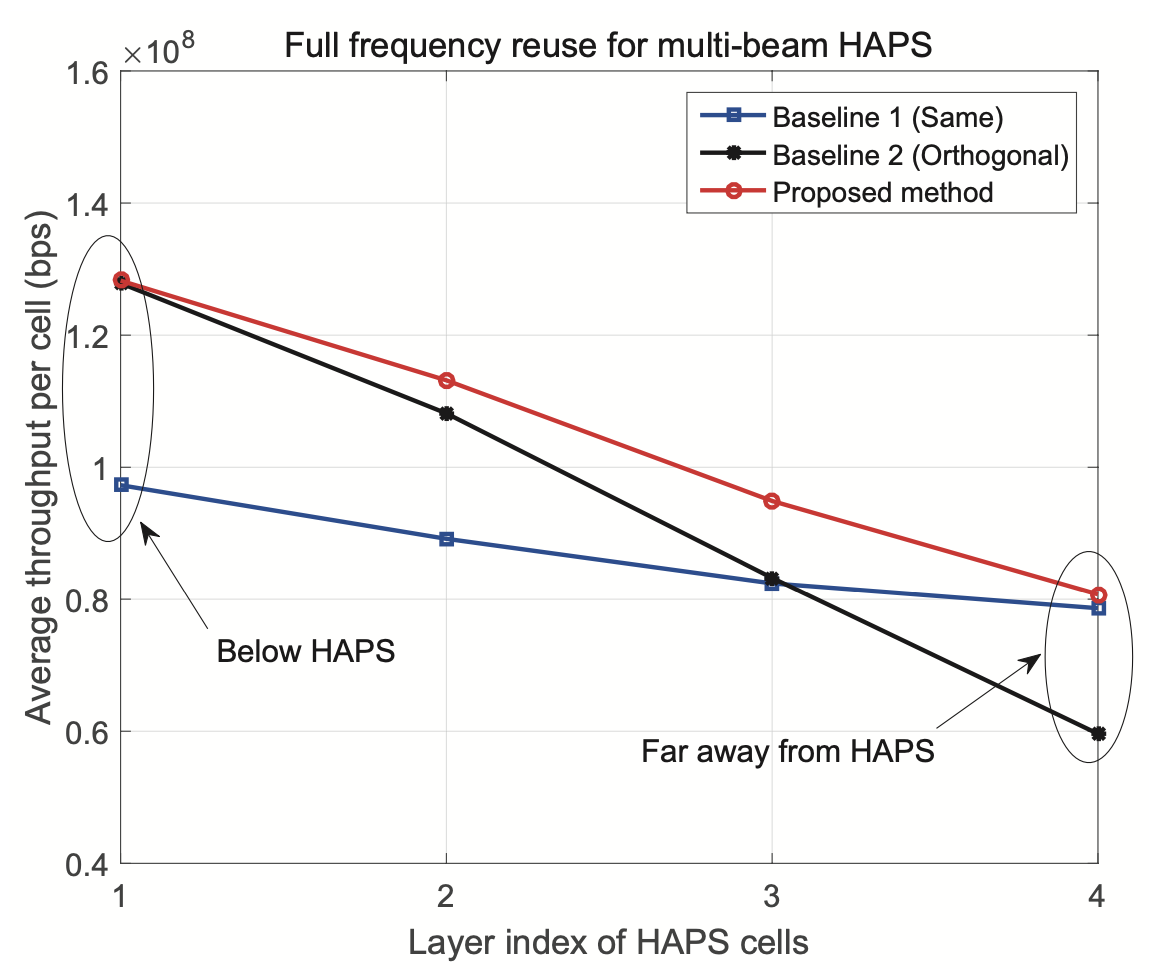
\includegraphics[width=0.5\textwidth]{05_avg-thruput-full-freq.png}
\caption[Average throughput with full frequency reuse in HAPS]{Average throughput per cell versus different layer index of HAPS cells with full frequency reuse in HAPS} \label{fig:05-avg-thruput-full-freq} 
\end{figure}

\begin{figure}[!hbp]
\centering
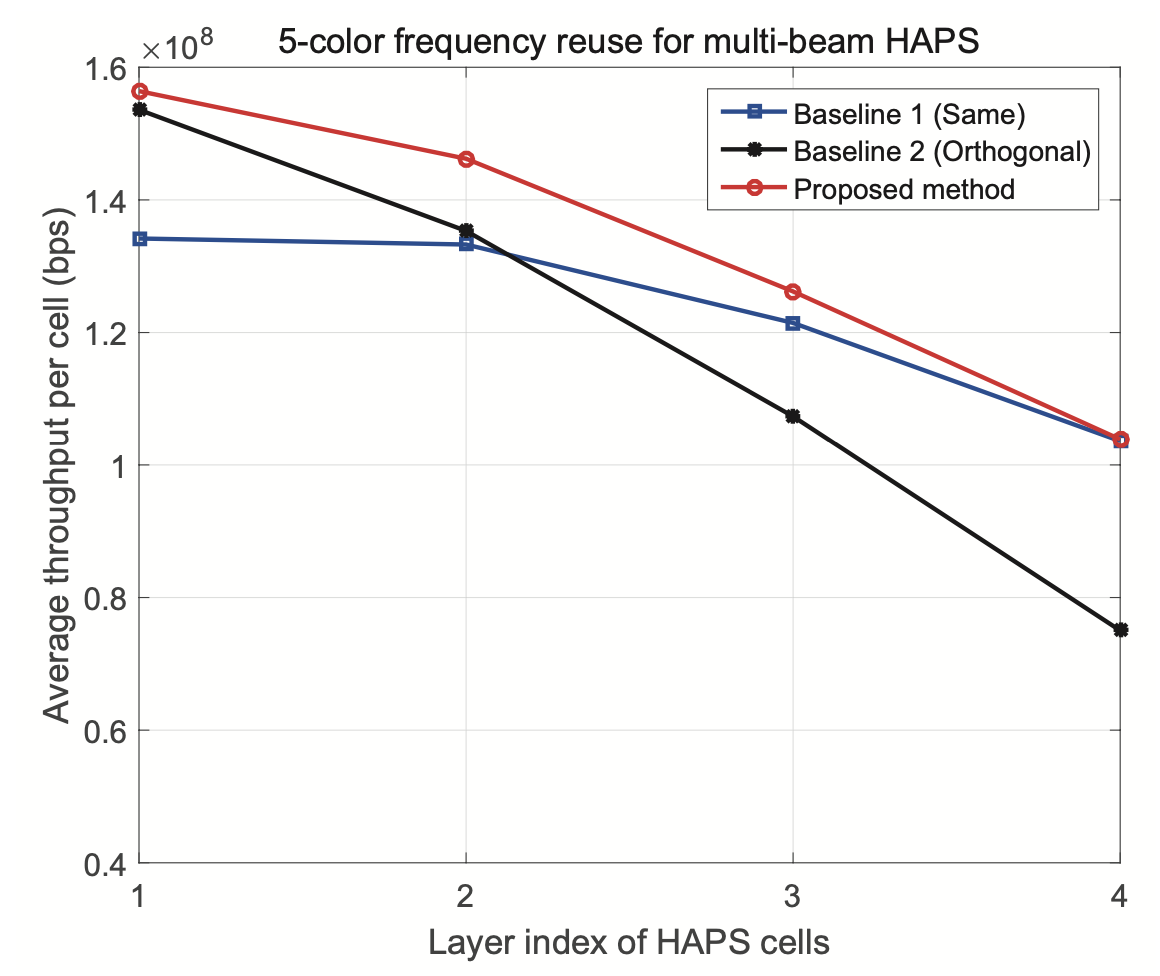
\includegraphics[width=0.5\textwidth]{05_avg-thruput-5-cl-freq.png}
\caption[Average throughput with 5-color frequency reuse in HAPS]{Average throughput per cell versus different layer index of HAPS cells with 5-color frequency reuse in HAPS} \label{fig:05-avg-thruput-5-cl-freq} 
\end{figure}
